\documentclass[11pt]{article}
\usepackage{amsmath,amssymb,fancyhdr,url,graphicx,courier,xcolor,multicol,listings,tikz}
\usepackage[top=1in,bottom=1in,left=0.75in,right=0.75in,headheight=.75in]{geometry}
\usepackage[small,bf]{caption}
\definecolor{shadethmcolor}{rgb}{0.96,0.96,0.96}
\pagestyle{fancy}
\lhead{T.~Keller, Y.~Tan, K.~Huang, and C.~Li}
\rhead{CSCI 6360 Group Project}
\cfoot{\thepage/\pageref{LastPage}}
\frenchspacing
%%%%%%%%%%%%%%%%%%%%%%%%%%%%%%%%%%%%%%%%%%%%%%%%%%%%%%%%%%%%%%%%%%%%%%%%%%%%%%%%%%%%%%%%%%%%%%%%%%%%
\definecolor{codebg}{gray}{0.8}
\renewcommand{\headrulewidth}{0.01in} \renewcommand{\footrulewidth}{0.01in}
\newcommand{\code}[1]{\colorbox{codebg}{\texttt{\footnotesize{#1}}}}
\lstset{language=C++,basicstyle=\footnotesize\ttfamily,language=bash,backgroundcolor=\color{codebg},xleftmargin=0pt,breaklines=true,alsoletter={--,/,[,=},alsodigit={-},showstringspaces=false,breakindent=0em,prebreak={ \textbackslash},postbreak={\phantom{m}}}
\usetikzlibrary{arrows,calc,backgrounds}
\tikzstyle{na} = [rectangle,draw=black,anchor=west]
\tikzstyle{nb} = [rectangle,draw=blue,anchor=west]
\tikzstyle{nz} = [rectangle,draw=red,anchor=west]

\tikzstyle{rank} = [draw,anchor=north,minimum size=2em]
\tikzstyle{mblock} = [draw,anchor=north,fill=black!20!white,minimum width=2em,minimum height=0.5em]
\tikzstyle{hblock} = [draw,anchor=north,fill=blue!20!white,minimum width=2em,minimum height=0.5em]
\tikzstyle{zblock} = [draw,anchor=north,fill=red!20!white,minimum width=2em]
%%%%%%%%%%%%%%%%%%%%%%%%%%%%%%%%%%%%%%%%%%%%%%%%%%%%%%%%%%%%%%%%%%%%%%%%%%%%%%%%%%%%%%%%%%%%%%%%%%%%
\begin{document}
\centerline{\LARGE{\bfseries MMSP Compute and I/O Performance on AMOS}}
\begin{multicols}{4}\centering
 \textbf{Trevor Keller}\\
 \emph{Materials Science}
 
 \textbf{Yixuan Tan}\\
 \emph{Mechanical Engineering}

 \textbf{Kun Huang}\\
 \emph{Physics}
 
 \textbf{Congrui Li}\\
 \emph{Computer Science}

\end{multicols}

\begin{center}
\texttt{\{kellet,tany3,huangk4,lic10\}@rpi.edu}

\vskip\baselineskip
Rensselaer Polytechnic Institute\\110 Eighth Street\\Troy, NY 12180

\vskip\baselineskip
May 8, 2014
\end{center}


\begin{abstract}
\noindent Parallel computing is a key capability for numerical models of physical systems.
Our group is interested specifically in the problem of grain growth in 3-dimensional polycrystalline metals.
Using the knowledge we gained in CSCI-6360, we have upgraded an existing research code, the Mesoscale Microstructure Simulation Project (MMSP), to use pthreads for computational performance gains and MPI-IO for parallel output of checkpoint files.
We discuss the speedup and bandwidth results, with recommendations for the ``best'' simulation conditions.

Our code is available online via \url{https://github.com/fifthblackbird/PPCproject}, and will be integrated into MMSP in the near future.
\end{abstract}

\begin{multicols*}{2}
\section{Introduction}
The Mesoscale Microstructure Simulation Project (MMSP) is a C++ code for parallel simulation of physical systems using Monte Carlo, phase-field, and similar methods.\footnote{\url{http://matforge.org/mmsp} and \url{http://github.com/mesoscale/mmsp}}
MMSP implements a 3-dimensional grid class, with back-end support for parallel synchronization and file I/O using MPI.
This grid facilitates computation of spatial derivatives by exchanging ``ghost'' cells between spatially adjacent ranks:
essentially, each face of the local 3-D grid needs to be sent to the MPI rank sharing that face.
This is a common feature of codes for numerical integration of partial differential equations;
indeed, while designed for materials science, MMSP could be applicable to a large number of numerical computing tasks.

To date, MMSP has been tested and used extensively on workstation-class machines, occasionally on clusters (such as the CCI Opteron cluster), and almost never on supercomputers.
Past efforts at MPI-IO have used \texttt{MPI\_File\_iwrite\_shared} and \texttt{MPI\_File\_iwrite\_at}, with default (\texttt{MPI\_NULL}) hints.
The code had not previously taken the underlying filesystem into consideration.
On AMOS, the GPFS has a blocksize of 8MB, while the MPI ranks may only write a few KB each.
This produced contention for a common GPFS block between thousands of processors and, ultimately, failure to write anything at all.
We chose to address this problem by implementing an explicit two-stage accumulate-and-write output function, wherein a few MPI ranks gather data from the upstream ranks that would contend for the same block;
only the accumulator ranks write to disk, once their output buffers are full.


\section{Algorithms\label{sec:algo}}
We selected two strong-scaling grain growth models -- Potts Monte Carlo and phase-field -- for comparison.

\subsection*{Voronoi Tessellation\label{sec:pvt}}
3-D simulations need a starting point, and the Poisson-Voronoi tessellation is the most common for grain growth simulations.
These tessellations are the combination of a Poisson point process for generating random seed points, followed by the Voronoi tessellation of space around those seeds;
that is to say, any point in space closer to one seed than any other belongs to that seed's domain.
This is done using the algorithm in Listing~\ref{lst:voro}, for a mesh containing $N$ nodes; it is a na\"ive algorithm, but easy to parallelize.
Since the Voronoi tessellation is embarassingly parallel, we chose not to devote resources to improving this implementation.
We did, however, modify the reference algorithm in the following ways:
\begin{enumerate}
 \item Instead of an \texttt{MPI\_Allgather} over every MPI rank, we determined which ranks were adjacent along a domain face or through a domain corner, and retrieved seeds from those ranks, only.
 \item We implemented pthreads by subdividing the loop \code{for (n=0; n<N; n++)} among the available threads, \code{for (n=nlo; n<nhi; n++)} with \texttt{nlo}$\geq0$ and \texttt{nhi<N} defined for each thread.
 \item Instead of the built-in random number generator, we generate seeds with the Mersenne twister.
\end{enumerate}
This reduced the runtime from $\mathcal{O}(2\ \mathrm{hours})$ to under a minute.
The final result of a Voronoi tessellation in 2-D ($1024^2$ mesh) performed on AMOS is provided in Fig.~\ref{fig:voro}.

\begin{center}\begin{minipage}{0.45\textwidth}\centering
  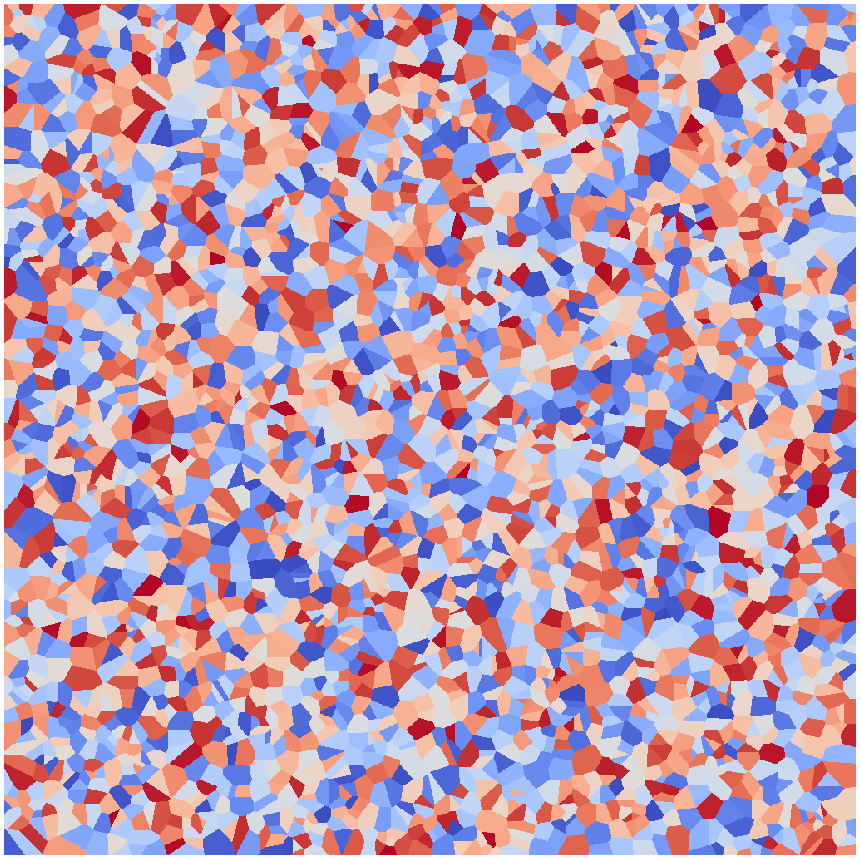
\includegraphics[width=\textwidth]{img/voronoi}
  \captionof{figure}{Voronoi tessellation produced by our code on AMOS ($1024\times1024$ mesh, $3336$ seeds; $1024$ threads). Runtime: 0.07 sec. Note the straight edges.\label{fig:voro}}
\end{minipage}\end{center}

\begin{minipage}{0.45\textwidth}
\begin{center}
\begin{lstlisting}
#include<cmath>
typedef struct {
  int x; int y; int z;
} int3;
void PVT(MMSP::grid& grid, int nseeds=10000)
{
  int np = MPI::COMM_WORLD.Get_size();
  while (nseeds%np != 0) ++nseeds;
  int S = nseeds/np;
  int3* seeds = new int3[S];
  int3* all_seeds = new int3[nseeds];
  for (i=0; i<nseeds; i++) {
    seeds[i].x=rand()%grid.xlength();
    seeds[i].y=rand()%grid.ylength();
    seeds[i].z=rand()%grid.zlength();
  }
  S *= 3;
  nseeds *= 3; 
  MPI_Allgather(seeds, S, MPI_INT, all_seeds, nseeds, MPI_INT, MPI_Comm_World);
  S /= 3;
  nseeds /= 3;
  for (n=0; n<N; n++) {
    int3 pos = MMSP::position(grid, n);
    int best;
    double min = std::pow(domain_size, 2);
    for (i=0; i<nseeds; i++) {
      dist = std::sqrt(std::pow(pos.x - seeds[i].x, 2) + std::pow(pos.y - seeds[i].y, 2) + std::pow(pos.z - seeds[i].z, 2))
      if (dist<min) {
	best = i;
	min=dist;
      }
    }
    grid(n) = best;
  }
  delete [] seeds;
  delete [] all_seeds;
}
\end{lstlisting}
\captionof{lstlisting}{Na\"ive Poisson-Voronoi tessellation algorithm.\label{lst:voro}}
\end{center}
\vskip\baselineskip
\end{minipage}


\subsection*{Potts Monte Carlo Model}
In a regular 2D or 3D lattice with N lattice sites, each site has \emph{n} neighbors. S$^0_\emph{i}$ is the grain ID at lattice site \emph{i}, where \emph{i}=1,\emph{N}. J is the grain boundary free energy per unit area between adjacent lattice sites. Then the total grain boundary energy of the system is:
\begin{equation}
E = \frac{J}{2}\sum_{i=1}^{N} \sum_{j=1}^{n} (1 - \delta_{S^0_\emph{i} S^j_\emph{i}})
\label{eqn:pottsE}
\end{equation}

where $\delta_{S^0_\emph{i} S^j_\emph{i}}$ is the Kronecker delta function (1 if $S^0_\emph{i}=S^j_\emph{i}$, 0 if $S^0_\emph{i} \neq S^j_\emph{i}$)

In serial, the Potts Monte Carlo algorithm is below:\\
(1) Q possible grain IDs.\\
(2) Randomly choose a site \emph{i}.\\
(3) Randomly choose a new grain ID at site \emph{i}.\\
(4) Compute the change in total system energy $\Delta E$\\
(5) The probability of accepting the new orientation is (Metropolis transition function)\\
\begin{equation}
p(\Delta E) = \begin{cases} 
		1 		   & \mathrm{if}\ \Delta E \le 0 \\
		\exp(-\Delta E/kT) & \mathrm{if}\ \Delta E > 0
	      \end{cases}
\label{eqn:pottsP}
\end{equation}
(6) One Monte Carlo Step (MCS) is defined as \emph{N} resetting grain ID attempts. \\

The serial Potts algorithm is not parallelizable for assigning each of P processors a subset of the loop iterations. This is because if step (2) is executed simultaneously on multiple processors, then two (or more) processors may pick adjacent (or the same) lattice sites. If this occurs, then when the two processors execute step (3), they will each attempt to flip the spin of their lattice site using incorrect information about neighboring spins (each other). This would violate the Monte Carlo rule of "detailed balance" which demands that two (or more) sites not be flipped simultaneously.

The parallelizable Potts Monte Carlo algorithm \cite{Wright,Shim} is to partion the overall grid  into different local grids so that each processor is assigned a contiguous subgrid. In two dimensions this is a small rectangular section, and in three dimensions it is a rectangular box. Each processor also stores a copy of the narrow strips (or planes in three dimensions) of lattice sites that immediately adjoin its sub-domain and which are actually owned by neighboring processors. 

This allows a processor to check neighboring spin values of sites on the edge of its sub-domain. With these data structures, every processor can now simultaneously flip spins in its sub-domain without violating the rule of detailed balance, so long as one processor does not choose a lattice site on an edge of its sub-domain at the same time the processor adjoining that edge does likewise. We enforce this restriction in our parallel Potts algorithm by "slicing" the subgrid as shown in Figure 1. lattice site is represented by a square (not the corners of the square) and assigned a ``sublattice'' number, 0 or 1.

A subgrid is divided into sublattices as in Figure 1, where only the lattice sites assigned to sublattice-0 are now shown as shaded.
The key point is that the 2 neighbors of a sublattice-0 lattice site do not include any other sublattice-0 lattice sites.
The parallel Monte Carlo Potts grain growth algorithm for one sweep can now be written as follows:

\begin{minipage}{0.475\textwidth}
\begin{center}
\begin{lstlisting}
in each processor
number of subgrids = number of pthreads;
n=2; // number of sublattice
  in subgrid-m (1=<m<=number of subgrids)
  {
    sublattice-1 = {sites with even x coordinates};
    sublattice-2 = {sites with odd x coordinates};  
  }
  in pthread-k with subgrid-k (1=<k<=number of pthreads)
  {
    for (i=1; i<=n; i++)
    { 
      for (j = 1; j<=number of sites in sublattice-i; j++)
      {
        Pick a site in sublattice-i randomly;
        Flip the grain ID to be a random value of its neighbors';
        Compute the change of total system energy;
        Accept or reject the change based on the Boltzmann criterion as in serial algorithm step (5);
      }
      Exchange grain IDs of boundary sites with neighboring processors;
    }
  }
}
\end{lstlisting}
\captionof{lstlisting}{Monte Carlo algorithm.\label{lst:mc}}
\end{center}
\vskip\baselineskip
\end{minipage}

This algorithm works for both 2-D and 3-D grid. Also, the communication of subgrid ``edges'' becomes ``planes'' in 3-D. 
This algorithm is not embarassingly parallel for the following aspects:\\
(1) Information on neighboring processors affects physics of the local processor. \\
(2) There are communications among neighboring subgrids.\\
(3) Threads are added into the flipping of grain ID of points.

\begin{center}
\begin{minipage}{0.475\textwidth}\centering
  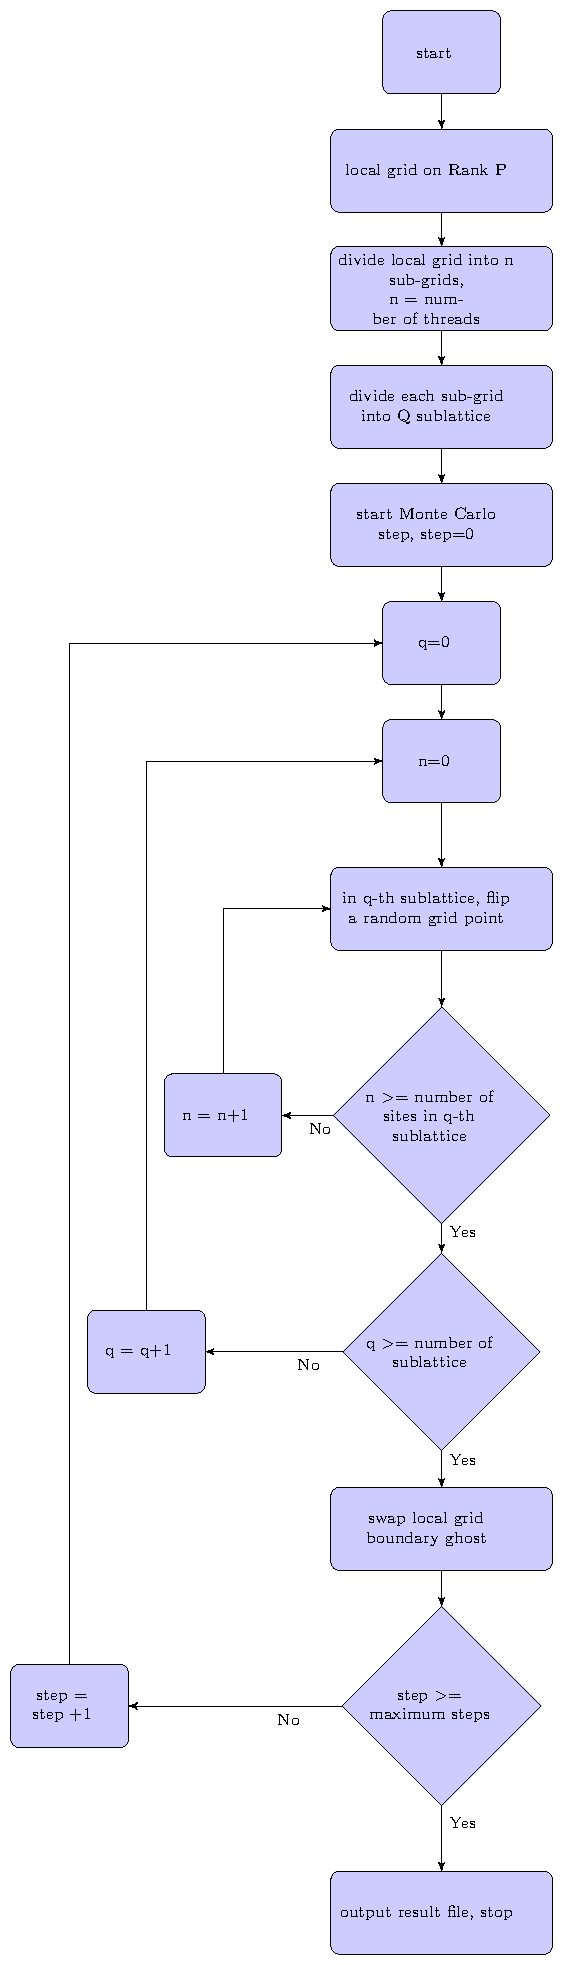
\includegraphics[height=7.25in]{flow_chart.pdf}
  \captionof{figure}{Flowchart of parallel Potts Monte Carlo algorithm.\label{fig:mc2}}
\end{minipage}
\end{center}

\begin{center}
\begin{minipage}{0.475\textwidth}\centering
  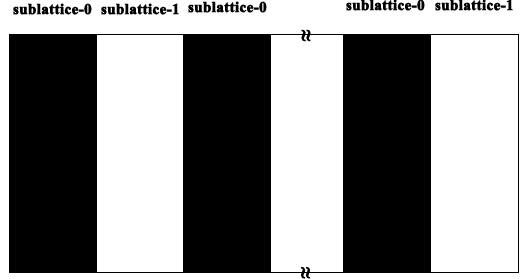
\includegraphics[height=1.75in]{img/mc-fig-01}
  \captionof{figure}{Slicing subgrid into sublattice used for parallel Potts grain growth algorithm.\label{fig:mc1}}
\end{minipage}
\end{center}

An example of 2-D grain growth using the Potts Monte Carlo physical model is given in Fig.~\ref{fig:voroggmc}.

\begin{center}\begin{minipage}{0.45\textwidth}\centering
  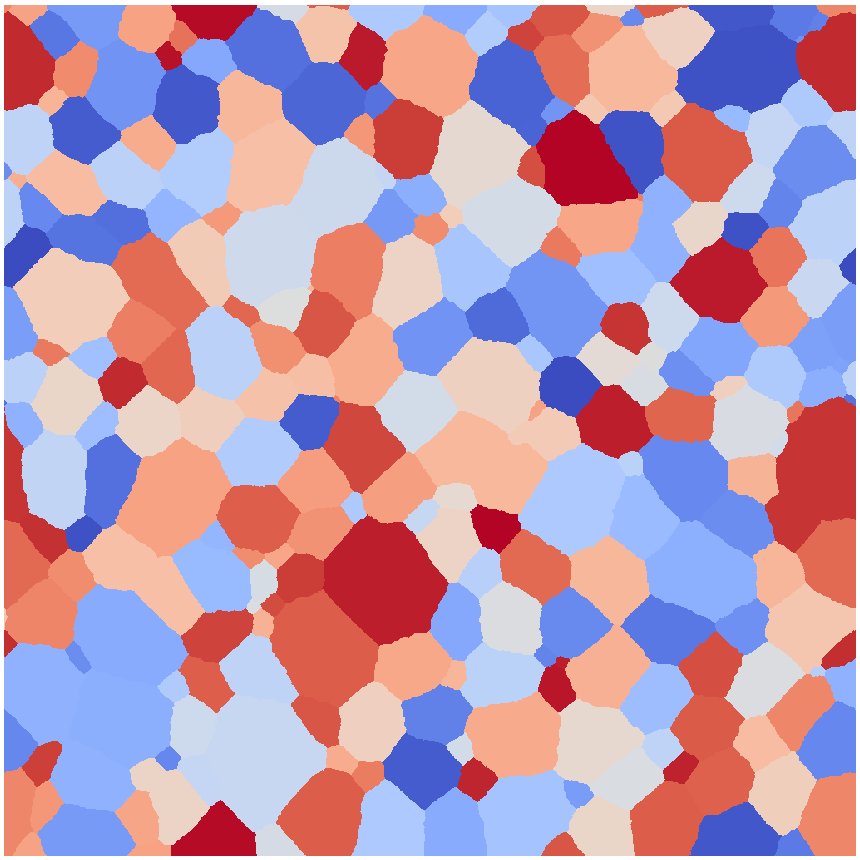
\includegraphics[width=\textwidth]{img/graingrowth-mc}
  \captionof{figure}{Grain growth produced by our phase-field code on AMOS ($5000$ iterations, $1024$ threads). Runtime: 18 minutes. Note the curved edges.\label{fig:voroggmc}}
\end{minipage}\end{center}


\subsection*{Phase-Field Model}
Phase-field models are useful for mesoscale simulations of cellular materials:
the models have a characteristic length scale $\mathcal{O}(1\ \mu\mathrm{m})$, with ``cells'' distinguished by some characteristic such as solid fraction (instead of liquid), magnetic field alignment, or grain orientation.
The interfaces between adjacent cells are modeled through the smooth, continuous transition of an order parameter $\phi$ between one (existence) and zero (absence).
The model implemented for this project assigns one order parameter to each grain, and each node in the computational mesh contains a sparse vector $\{\phi\}$, ranging in size between one and 27 entries (in 3-D) \cite{Steinbach1999}.
Grain growth in these simulations occurs by numerically integrating the parabolic partial differential equation-of-motion,
\begin{align}
\frac{\partial\phi_i}{\partial t} = -\frac{\mu}{S}\sum\limits_{j\neq i}^S\Bigg[
  &\sum\limits_{k\neq i}^S\bigg(\frac{1}{2}\varepsilon^2\nabla^2\phi_k+\omega|\phi_k|\bigg)\notag\\
  -&\sum\limits_{\ell\neq j}^S\bigg(\frac{1}{2}\varepsilon^2\nabla^2\phi_\ell+\omega|\phi_\ell|\bigg)\Bigg],\label{eqn:pf}
\end{align}
using information from the $S$-dimensional sparse vector $\{\phi\}$ at each point, with interfacial mobility $\mu$ and model parameters $\varepsilon$ and $\omega$.
The Laplacian operator $\nabla^2 = \frac{\partial^2}{\partial x^2} + \frac{\partial^2}{\partial y^2} + \frac{\partial^2}{\partial z^2}$;
in each dimension, the Laplacian operator for a given order parameter is
\begin{equation}
\frac{\partial^2\phi}{\partial x^2} \approx \frac{\Delta(\Delta\phi)}{\Delta x^2} = \frac{\phi_{i+1} - 2\phi_i + \phi_{i-1}}{2\Delta x^2},\label{eqn:laplacian}
\end{equation}

where the values $\phi_{i+1}$ and $\phi_{i-1}$ are read from the two neighbors of point $i$. 
These second-order spatial derivatives are the reason this is not an embarassingly parallel algorithm.
At the boundary of the grid stored on each MPI rank, values of $\phi_{i \in S}$ must be set in \emph{ghost cells} with data retrieved from the adjacent grid.
The more MPI ranks, the more ghost data, and the higher the network load.
This intercommunication of boundary values occurs after each numerical integration iteration; that is to say, the serial computation and parallel data synchronization occur at different times.
Listing~\ref{lst:pf} summarizes the phase-field algorithm as-implemented for $T$ timesteps on a local grid containing $N$ nodes, using only one thread per MPI rank.
\begin{minipage}{0.475\textwidth}
\begin{center}
\begin{lstlisting}
void initialize(MMSP::grid);
MMSP::sparse update(MMSP::grid, int);
void ghostswap(MMSP::grid);
void swap(MMSP::grid, MMSP::grid);

int main()
{
  MMSP::grid pfgrid;
  MMSP::grid newgrid;
  PVT(pfgrid);
  for (t=0; t<T; t++) {
    ghostswap(pfgrid);
    for (n=0; n<N; n++)
      newgrid(n) = update(pfgrid, n);
    swap(pfgrid, newgrid);
  }
  return 0;
}
\end{lstlisting}
\captionof{lstlisting}{Phase-field algorithm. \texttt{PVT()} was given in Listing~\ref{lst:voro}; \texttt{update()} implements Eqn.~\ref{eqn:pf}.\label{lst:pf}}
\end{center}
\vskip\baselineskip
\end{minipage}

The independence of computation from communication and the increasing communication overhead associated with adding MPI ranks makes pthreading a favorable approach for maximizing performance in this model.
To use pthreads, Listing~\ref{lst:pf} is modified simply to loop over \code{n=nlo; n<nhi; n++}, with \texttt{nlo}$\geq0$ and \texttt{nhi}$<$\texttt{N} defined for each pthread.

An example of 2-D grain growth using the phase-field physical model is given in Fig.~\ref{fig:vorogg}.

\begin{center}\begin{minipage}{0.45\textwidth}\centering
  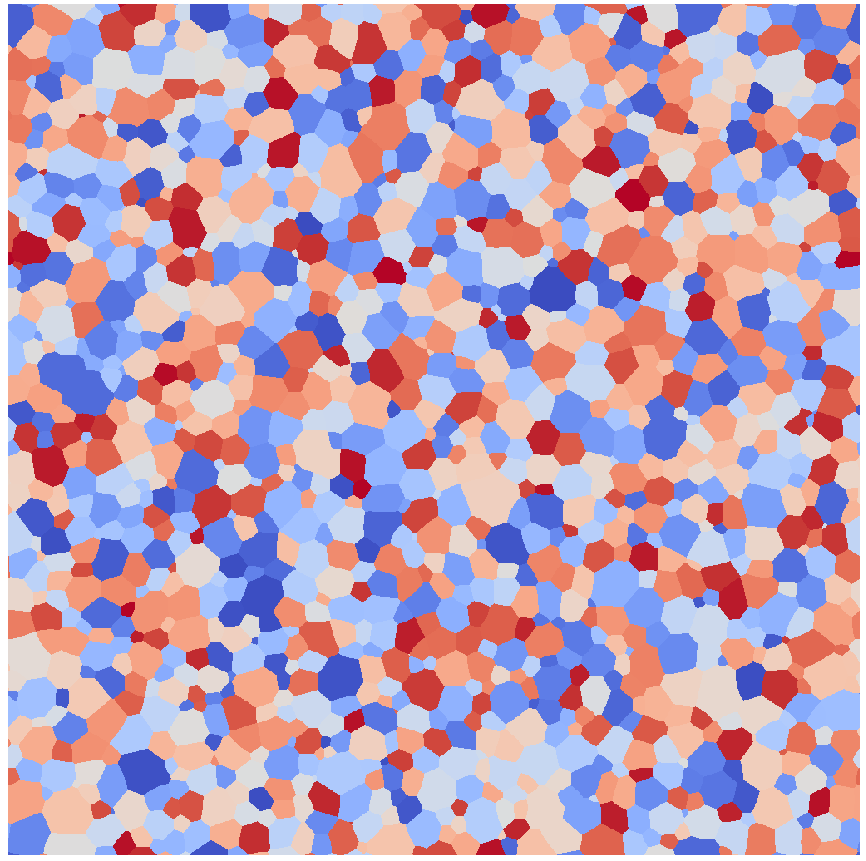
\includegraphics[width=\textwidth]{img/graingrowth}
  \captionof{figure}{Grain growth produced by our phase-field code on AMOS ($5000$ iterations, $1024$ threads). Runtime: 13 minutes. Note the curved edges.\label{fig:vorogg}}
\end{minipage}\end{center}

\subsection*{Two-Step I/O}
MMSP data files are intended for checkpoint and visualization purposes.
Each file is written with a human-readable header, followed by a direct dump of the local grid from each MPI rank.
For reference, the MMSP file structure is presented in Fig.~\ref{fig:file}.
Since the MMSP grid can grow fairly large, \texttt{zlib} compression is used on-the-fly;
For 3-D simulations on reasonably large meshes, the compressed file sizes range between $10$ MB for the initial condition to $3$ GB for intermediate stages of grain growth.

The stock MMSP distribution comes with an \texttt{output} function which synchronizes data sizes across all MPI ranks, sets a local offset, then calls \texttt{MPI\_File\_iwrite\_at} with a matching \texttt{MPI\_Wait}.
The function is represented schematically in Fig.~\ref{fig:stockio}, with $8$ MPI ranks writing roughly $17$ MB of data, or $2.125$ blocks on the GPFS.
This filesize is typical for Poisson-Voronoi tessellations on 3-D meshes of $512^3$ nodes, storing an \texttt{int} or \texttt{float} at each node.
The function works nicely for relatively low levels of parallelization:
as depicted, with a handful of ranks, there is only modest contention for common blocks on the filesystem.
On the CCI Opteron cluster, 3-D meshes of $400^3$ nodes wrote to disk on up to $192$ MPI ranks.
However, the stock function has never worked on our Blue Gene systems:
neither the Blue Gene/P nor AMOS ever wrote a complete MMSP file to disk.
In the rare case when the file had non-zero size, it was too small by an integer multiple of the size-per-rank expected:
some ranks were simply barred from contributing to the file.

Our working hypothesis for AMOS's failure to write is that dividing the smaller files among thousands of processors created extreme contention for common blocks on the parallel filesystem, or else multiple GPFS servers attempted to allocate space for the same block.
For a typical simulation on AMOS, each block would receive write requests from $\mathcal{O}(100)$ ranks.
Past experience suggests this is beyond ROMIO's capacity to smoothly handle.

We have resolved the critical file I/O conflict by implementing a two-stage approach:
a set of MPI ranks equal to the number of filesystem blocks to be written are labelled ``aggregators,'' and each initializes a filesystem-block-sized buffer with a chunk of local data at the root.
Non-aggregators send data to the aggregator immediately downstream, using \texttt{MPI\_Isend}.
Once the file buffers are full, the aggregators write to disk.
The procedure is represented schematically in Fig.~\ref{fig:bgqio}.
%It was designed to minimize data transmission by keeping the largest amount of data local to each aggregator as possible.
The approach is similar to the ``reduced blocking I/O'' used in PHASTA \cite{Carothers2010,Carothers2011}.


\begin{minipage}{0.475\textwidth}
\begin{center}
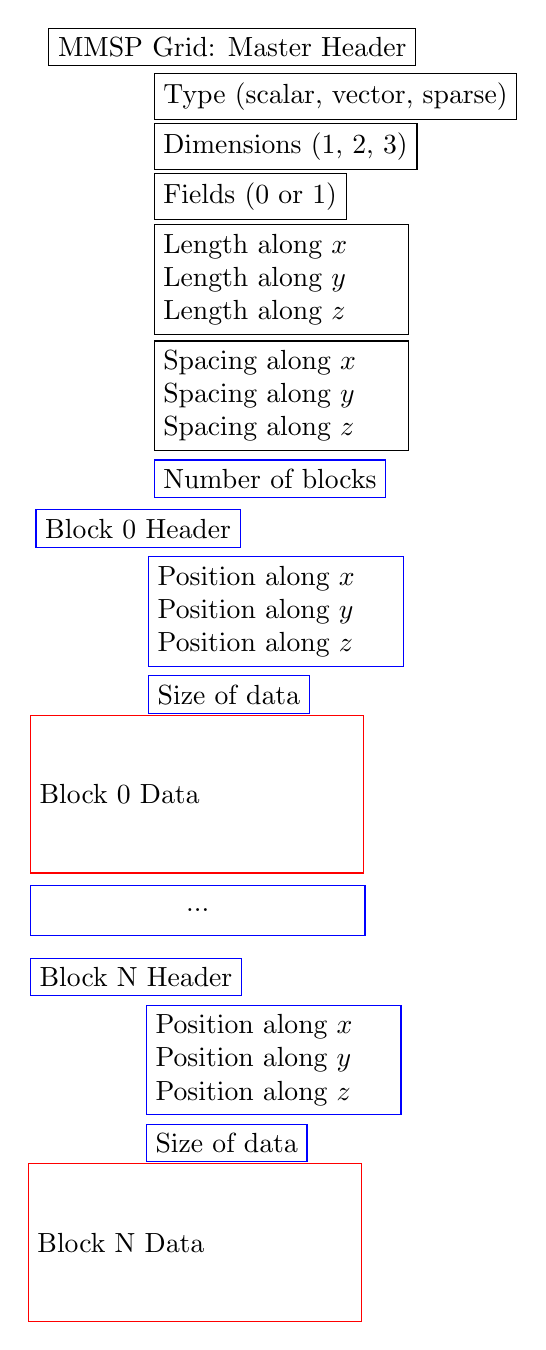
\begin{tikzpicture}[scale=0.5]
  \node[na](gh){MMSP Grid: Master Header};
  \node[na] at ($(gh)+(-2,-3\baselineskip)$) {Type (scalar, vector, sparse)};
  \node[na] at ($(gh)+(-2,-6\baselineskip)$) {Dimensions (1, 2, 3)};
  \node[na] at ($(gh)+(-2,-9\baselineskip)$) {Fields (0 or 1)};
  \node[na,text width=3cm] at ($(gh)+(-2,-14\baselineskip)$) {Length along $x$ Length along $y$ Length along $z$};
  \node[na,text width=3cm] at ($(gh)+(-2,-21\baselineskip)$) {Spacing along $x$ Spacing along $y$ Spacing along $z$};
  \node[nb] at ($(gh)+(-2,-26\baselineskip)$) {Number of blocks};
  \node[nb](sh) at ($(gh)+(-5,-29\baselineskip)$) {Block 0 Header};
  \node[nb,text width=3cm] at ($(sh)+(0.25,-5\baselineskip)$) {Position along $x$ Position along $y$ Position along $z$};
  \node[nb] at ($(sh)+(0.25,-10\baselineskip)$) {Size of data};
  \node[nz,minimum height=2cm,text width=4cm] at ($(sh)+(-2.75,-16\baselineskip)$) {Block 0 Data};
  \node[nb,minimum height=1.5\baselineskip,minimum width=4.25cm] at ($(sh)+(-2.75,-23\baselineskip)$) {...};
  \node[nb](sn) at ($(sh)+(-2.75,-27\baselineskip)$) {Block N Header};
  \node[nb,text width=3cm] at ($(sn)+(0.25,-5\baselineskip)$) {Position along $x$ Position along $y$ Position along $z$};
  \node[nb] at ($(sn)+(0.25,-10\baselineskip)$) {Size of data};
  \node[nz,minimum height=2cm,text width=4cm] at ($(sn)+(-2.75,-16\baselineskip)$) {Block N Data};
\end{tikzpicture}
\captionof{figure}{MMSP checkpoint file format. Fields surrounded by black boxes are ASCII, blue are binary, red are \texttt{zlib}-compressed binary.\label{fig:file}}
\end{center}
\vskip\baselineskip
\end{minipage}


\begin{minipage}{0.45\textwidth}
\begin{center}
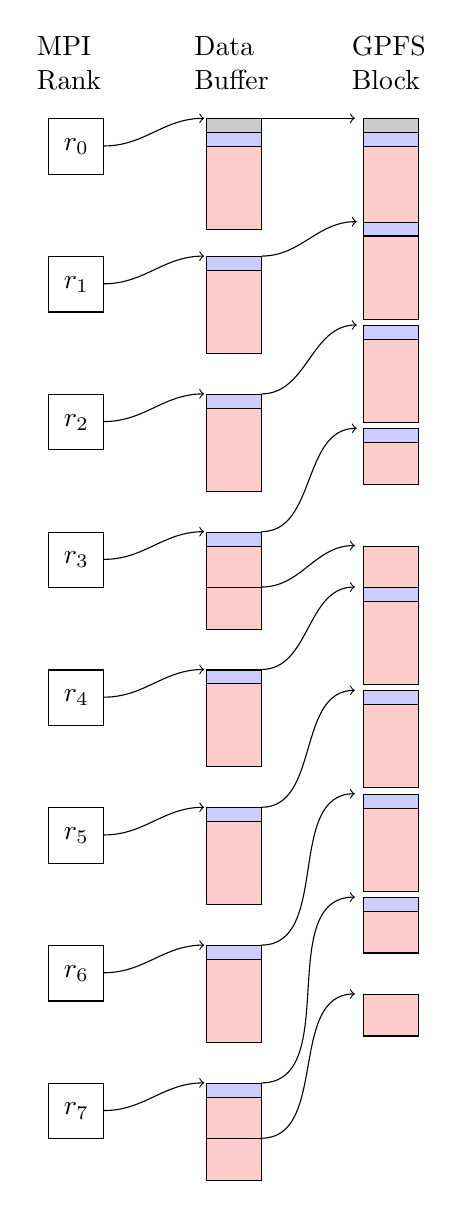
\begin{tikzpicture}[scale=0.5]
  % Column titles
  \node[text width=1cm] at (0,0) {MPI Rank};
  \node[text width=1cm] at (4,0) {Data Buffer};
  \node[text width=1cm] at (8,0) {GPFS Block};
  \foreach \y in {0,1,2,3,4,5,6,7} {
    \node[rank] at ($(0,-4em)+(0,-3.5*\y)$) {$r_\y$};
  }
  % Data buffers
  \node[mblock] at (4,-4em) { };
  \node[hblock] at (4,-5em) { };
  \node[zblock,minimum height=3em] at (4,-6em) { };
  \path[->,out=0,in=180] (2em,-6em) edge (3.25,-4em);
  \foreach \y in {1,2,3,4,5,6,7} {
    \node[hblock] at ($(4,-4em)+(0,-3.5*\y)$) { };
    \node[zblock,minimum height=3em] at ($(4,-5em)+(0,-3.5*\y)$) { };
    \path[->,out=0,in=180] ($(2em,-6em)+(0,-3.5*\y)$) edge ($(3.25,-4em)+(0,-3.5*\y)$);
  }
  \node[zblock,minimum height=1.5em] at ($(4,-8em)+(0,-3.5*3)$) { };
  \node[zblock,minimum height=1.5em] at ($(4,-8em)+(0,-3.5*7)$) { };
  % GPFS blocks
  \node[mblock] at (8,-4em) { };
  \node[hblock] at (8,-5em) { };
  \node[zblock,minimum height=3em] at (8,-6em) { };
  \path[->] ($(2em,-4em)+(4,0)$) edge ($(2em,-4em)+(6.375,0)$);
  \foreach \y in {1,2,3} {
    \node[hblock] at ($(8,-4em)+(0,-2.625*\y)$) { };
    \path[->,out=0,in=180] ($(2em,-4em)+(4,-3.5*\y)$) edge ($(7.125,-4em)+(0,-2.625*\y)$);
  }
  \node[zblock,minimum height=1.5em] at ($(8,-5em)+(0,-2.625*3)$) { };
  \node[zblock,minimum height=1.5em] at ($(8,-5em)+(0,-2.625*4)$) { };
  \path[->,out=0,in=180] ($(2em,-8em)+(4,-2.625*4)$) edge ($(2em,-5em)+(6.375,-2.625*4)$);
  \foreach \y in {1,2} {
    \node[zblock,minimum height=3em] at ($(8,-5em)+(0,-2.625*\y)$) { };
  }
  \foreach \y in {4,5,6,7} {
    \node[hblock] at ($(8,-8em)+(0,-2.625*\y)$) { };
    \path[->,out=0,in=180] ($(2em,-4em)+(4,-3.5*\y)$) edge ($(2em,-8em)+(6.375,-2.625*\y)$);
  }
  \foreach \y in {4,5,6} {
    \node[zblock,minimum height=3em] at ($(8,-9em)+(0,-2.625*\y)$) { };
  }
  \node[zblock,minimum height=1.5em] at ($(8,-9em)+(0,-2.625*7)$) { };
  \node[zblock,minimum height=1.5em] at ($(8,-15em)+(0,-2.625*7)$) { };
  \path[->,out=0,in=180] ($(2em,-8em)+(4,-3.5*7)$) edge ($(2em,-15em)+(6.375,-2.625*7)$);
\end{tikzpicture}
\captionof{figure}{Schematic of data movement in stock \texttt{MMSP::output()} function, implemented using explicit offsets and \texttt{MPI\_File\_iwrite\_at}. Colors have the same meaning as in Fig.~\ref{fig:file}. In this example, each MPI rank writes to disk. The filesize is slightly larger than two GPFS blocks, a common situation when writing initial conditions. For massively parallel systems, such as AMOS, this scenario overtaxes the GPFS backend.\label{fig:stockio}}
\end{center}
\vskip\baselineskip
\end{minipage}

\begin{minipage}{0.45\textwidth}
\begin{center}
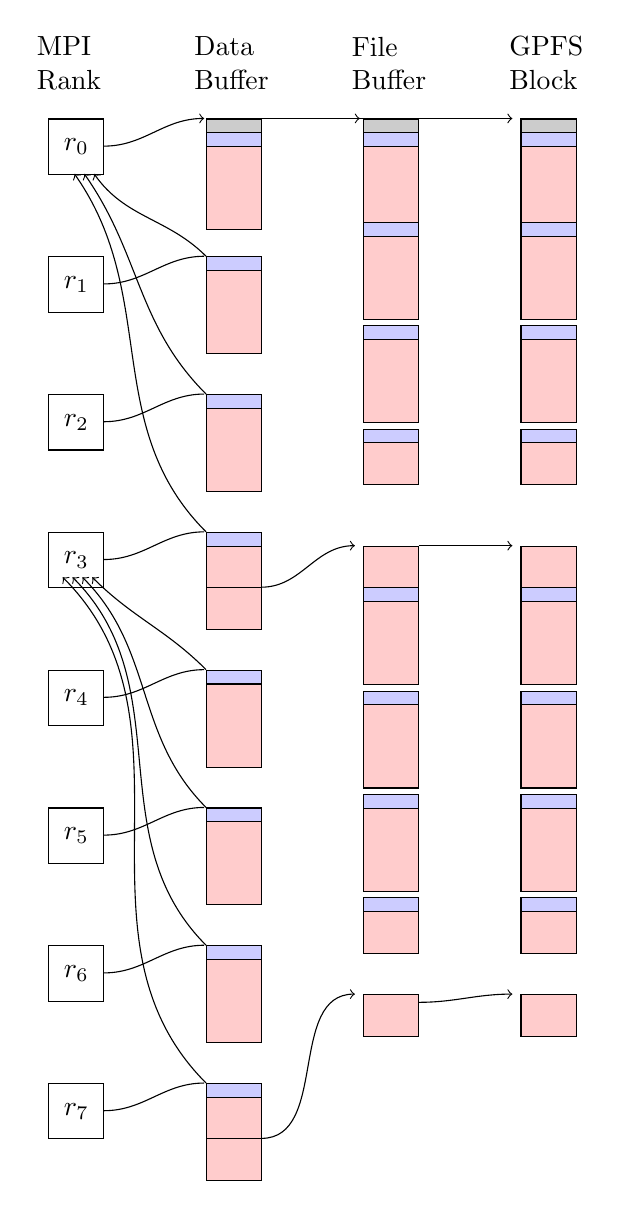
\begin{tikzpicture}[scale=0.5]
  % Column titles
  \node[text width=1cm] at (0,0) {MPI Rank};
  \node[text width=1cm] at (4,0) {Data Buffer};
  \node[text width=1cm] at (8,0) {File Buffer};
  \node[text width=1cm] at (12,0) {GPFS Block};
  \foreach \y in {0,1,2,3,4,5,6,7} {
    \node[rank] at ($(0,-4em)+(0,-3.5*\y)$) {$r_\y$};
  }
  % Data buffers
  \node[mblock] at (4,-4em) { };
  \node[hblock] at (4,-5em) { };
  \node[zblock,minimum height=3em] at (4,-6em) { };
  \path[->,out=0,in=180] (2em,-6em) edge (3.25,-4em);
  \foreach \y in {1,2,3,4,5,6,7} {
    \node[hblock] at ($(4,-4em)+(0,-3.5*\y)$) { };
    \node[zblock,minimum height=3em] at ($(4,-5em)+(0,-3.5*\y)$) { };
    \path[-,out=0,in=180] ($(2em,-6em)+(0,-3.5*\y)$) edge ($(3.25,-4em)+(0,-3.5*\y)$);
  }
  \node[zblock,minimum height=1.5em] at ($(4,-8em)+(0,-3.5*3)$) { };
  \node[zblock,minimum height=1.5em] at ($(4,-8em)+(0,-3.5*7)$) { };
  % File buffers
  \node[mblock] at (8,-4em) { };
  \node[hblock] at (8,-5em) { };
  \node[zblock,minimum height=3em] at (8,-6em) { };
  \path[->] ($(2em,-4em)+(4,0)$) edge ($(2em,-4em)+(6.5,0)$);
  \foreach \y in {1,2,3} {
    \node[hblock] at ($(8,-4em)+(0,-2.625*\y)$) { };
    \path[->,out=135,in=305] ($(-2em,-4em)+(4,-3.5*\y)$) edge ($(2em,-8em)+(-0.25*\y,0)$);
  }
  \node[zblock,minimum height=1.5em] at ($(8,-5em)+(0,-2.625*3)$) { };
  \node[zblock,minimum height=1.5em] at ($(8,-5em)+(0,-2.625*4)$) { };
  \path[->,out=0,in=180] ($(2em,-8em)+(4,-2.625*4)$) edge ($(2em,-5em)+(6.375,-2.625*4)$);
  \foreach \y in {1,2} {
    \node[zblock,minimum height=3em] at ($(8,-5em)+(0,-2.625*\y)$) { };
  }
  \foreach \y in {4,5,6,7} {
    \node[hblock] at ($(8,-8em)+(0,-2.625*\y)$) { };
    \path[->,out=135,in=315] ($(-2em,-4em)+(4,-3.5*\y)$) edge ($(4em,-14.75em)+(-0.25*\y,-2.625*3)$);
  }
  \foreach \y in {4,5,6} {
    \node[zblock,minimum height=3em] at ($(8,-9em)+(0,-2.625*\y)$) { };
  }
  \node[zblock,minimum height=1.5em] at ($(8,-9em)+(0,-2.625*7)$) { };
  \node[zblock,minimum height=1.5em] at ($(8,-15em)+(0,-2.625*7)$) { };
  \path[->,out=0,in=180] ($(2em,-8em)+(4,-3.5*7)$) edge ($(2em,-15em)+(6.375,-2.625*7)$);
  % GPFS blocks
  \node[mblock] at (12,-4em) { };
  \node[hblock] at (12,-5em) { };
  \node[zblock,minimum height=3em] at (12,-6em) { };
  \path[->] ($(2em,-4em)+(4,0)$) edge ($(2em,-4em)+(10.375,0)$);
  \foreach \y in {1,2,3} {
    \node[hblock] at ($(12,-4em)+(0,-2.625*\y)$) { };
  }
  \node[zblock,minimum height=1.5em] at ($(12,-5em)+(0,-2.625*3)$) { };
  \node[zblock,minimum height=1.5em] at ($(12,-5em)+(0,-2.625*4)$) { };
  \foreach \y in {1,2} {
    \node[zblock,minimum height=3em] at ($(12,-5em)+(0,-2.625*\y)$) { };
  }
  \path[->,out=0,in=180] ($(2em,-5em)+(8,-2.625*4)$) edge ($(2em,-5em)+(10.375,-2.625*4)$);
  \foreach \y in {4,5,6,7} {
    \node[hblock] at ($(12,-8em)+(0,-2.625*\y)$) { };
  }
  \foreach \y in {4,5,6} {
    \node[zblock,minimum height=3em] at ($(12,-9em)+(0,-2.625*\y)$) { };
  }
  \node[zblock,minimum height=1.5em] at ($(12,-9em)+(0,-2.625*7)$) { };
  \node[zblock,minimum height=1.5em] at ($(12,-15em)+(0,-2.625*7)$) { };
  \path[->,out=0,in=180] ($(2em,-8.125em)+(8,-3.5*6)$) edge ($(2em,-15em)+(10.375,-2.625*7)$);
\end{tikzpicture}
\captionof{figure}{Schematic of data movement in our two-stage aggregating \texttt{MMSP::output\_bgq()} function. Colors have the same meaning as in Fig.~\ref{fig:file}. In this example, MPI ranks 0, 3, and 7 are aggregators: the arrows from data buffers represent \texttt{MPI\_Isend}s from upstream MPI ranks, followed by \texttt{MPI\_File\_Iwrite\_at} from the aggregators, only. The smaller number of larger I/O requests are easily served by the GPFS backend.\label{fig:bgqio}}
\end{center}
\vskip\baselineskip
\end{minipage}


\newpage
\section{Results and Discussion}
Each node on AMOS contains a 17-core PowerPC A2 processor, of which 16 cores are accessible to MPI.
Each core provides hardware support for up to 4 threads, for a total capacity of 64 threads per node.
For the purposes of analyzing the performance of our code, we ran simulations using the Potts Monte Carlo and phase-field models described in Sec.~\ref{sec:algo} using the configurations given in Table~\ref{tab:cond}.
These conditions were chosen to reveal trends in compute performance (increased pthreading) and file I/O (increasing node count).
Column~4 in Table~\ref{tab:cond} represents the conserved quantity $np$ for each node count:
the number of MPI ranks is inversely proportional to the number of pthreads, and the ``total capacity'' for parallel work is held constant.


\begin{center}
\begin{minipage}{0.45\textwidth}\centering
\captionof{table}{Summary of execution conditions on AMOS. \checkmark indicates success, $\times$ failure to exit cleanly within the $30$-minute window.\label{tab:cond}}
\begin{footnotesize}
\bgroup
\renewcommand\tabcolsep{5pt}
\begin{tabular}{|cccc|cc|}\hline
AMOS  	& MPI 	& threads & Parallel	& Monte	& Phase\\
Nodes	& Ranks & per rank & Capacity	& Carlo	& Field\\
($N$)	& ($n$)	& ($p$)	& ($np$)	& result & result\\\hline
32	& 32	& 64	& 2048	&\checkmark &\checkmark \\
32	& 64	& 32	& 2048	&\checkmark &\checkmark \\
32	& 128	& 16	& 2048	&\checkmark &\checkmark \\
32	& 512	& 4	& 2048	&\checkmark &\checkmark \\
32	& 2048	& 1	& 2048	&\checkmark &\checkmark \\\hline
64	& 64	& 64	& 4096	&$\times$ &$\times$ \\
64	& 128	& 32	& 4096	&\checkmark &\checkmark \\
64	& 256	& 16	& 4096	&\checkmark &\checkmark \\
64	& 1024	& 4	& 4096	&\checkmark &\checkmark \\
64	& 4096	& 1	& 4096	&\checkmark &\checkmark \\\hline
128	& 128	& 64	& 8192	&$\times$ &$\times$ \\
128	& 256	& 32	& 8192	&\checkmark &\checkmark \\
128	& 1024	& 16	& 8192	&\checkmark &\checkmark \\
128	& 2048	& 4	& 8192	&\checkmark &\checkmark \\
128	& 8192	& 1	& 8192	&$\times$ &$\times$ \\\hline
256	& 256	& 64	& 16384	&$\times$ &$\times$\\
256	& 512	& 32	& 16384	&$\times$ &\checkmark \\
256	& 1024	& 16	& 16384	&\checkmark &\checkmark \\
256	& 4096	& 4	& 16384	&\checkmark &\checkmark \\
256	& 16384	& 1	& 16384	&$\times$ &$\times$ \\\hline
\end{tabular}
\egroup
\end{footnotesize}
\end{minipage}
\end{center}

For both physical models, we used a cubic 3-D mesh with $512$ nodes per edge, for a total of 134,217,728 nodes in the mesh.
These meshes were coarsened for fifteen steps (Monte Carlo steps or phase-field iterations), which is short, but still produced a representative result.
The major difference between the meshes is in the data type:
Monte Carlo meshes store one scalar value (the grain ID) at each node, while the phase-field mesh stores a set of order parameters (ranging in value between zero and one) at each node.

The Poisson-Voronoi tessellation (PVT) has nearly identical behavior for both meshes:
it either sets the scalar value, or sets to one the paramater corresponding to that scalar, at each mesh point.
As evident in Figs.~\ref{fig:vorot}~and~\ref{fig:vorob}, aside from a couple missing values due to pthreading limitations, the results are indistinguishable.
This suggests our implementations of the algorithm for both mesh types are correct, or at least consistent with each other.
The graphs show a minimum in compute time between 4--16 pthreads, with a sharp increase for $32$.
This is likely due to the overhead associated with spawning new pthreads, especially since increasing the number of threads must decrease the work available for each thread to perform.
Globally, the more MPI ranks available, the faster the initialization, since there is no such overhead associated with adding MPI ranks.
There is also a sharp maximum in write bandwidth between 4--16 threads, which is unexpected.
The intialization files are roughly 20 MB, or 2.2 blocks on the GPFS;
the fewer the threads, the more data transfer between the workers and the three aggregator ranks.
This peak is almost certainly due to data compression during output, which we did not pthread, but apparently should have:
\texttt{zlib} is an expensive algorithm.
The higher the number of pthreads, the fewer MPI ranks available to compress the data before writing to disk.

\begin{center}
\begin{minipage}{0.4\textwidth}\centering
  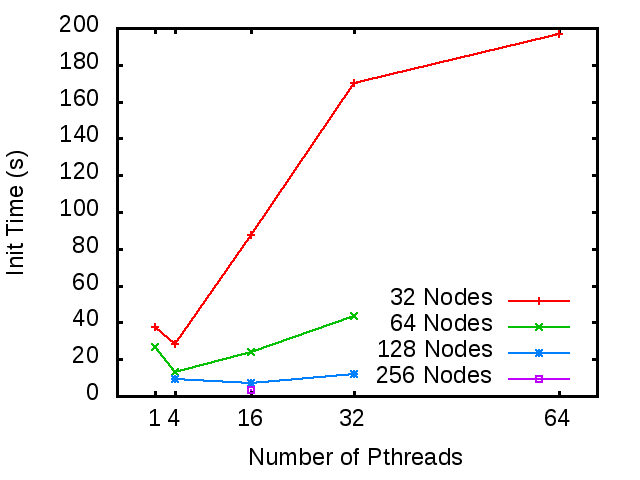
\includegraphics[width=\textwidth]{img/prMC-init}
  
  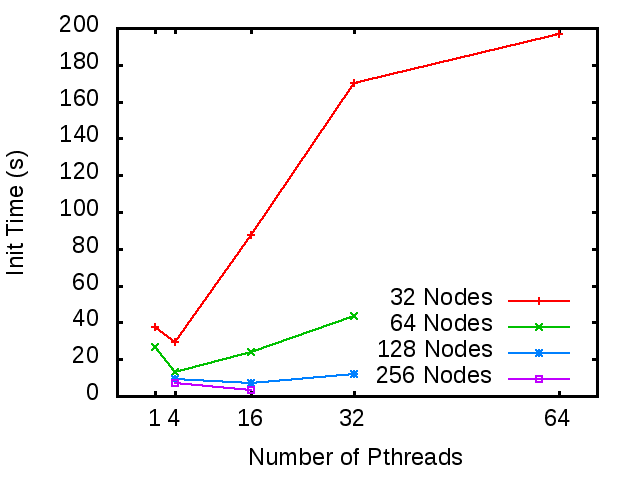
\includegraphics[width=\textwidth]{img/pr-init}
  \captionof{figure}{Initialization (PVT) time for (top) scalar-valued and (bottom) sparse vector-valued meshes.\label{fig:vorot}}
\end{minipage}
\end{center}

\begin{center}
\begin{minipage}{0.4\textwidth}\centering
  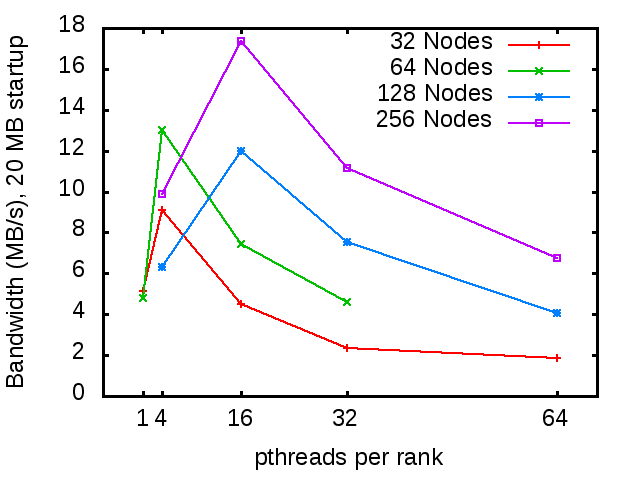
\includegraphics[width=\textwidth]{img/prMC-initBW}

  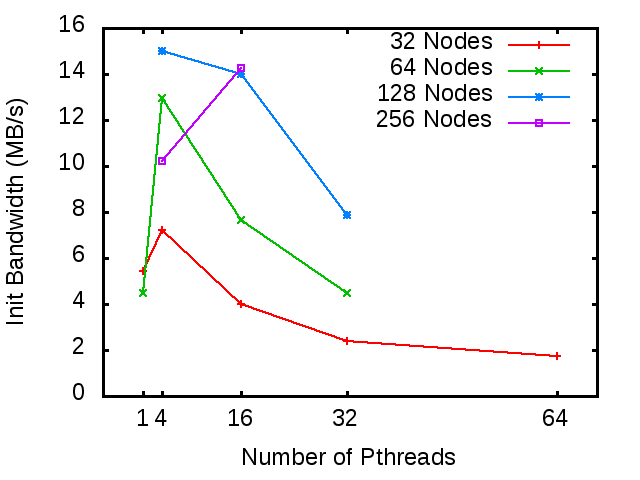
\includegraphics[width=\textwidth]{img/pr-initBW}
  \captionof{figure}{Parallel I/O bandwidth writing PVT-initialized (top) scalar-valued and (bottom) sparse-vector-valued meshes.\label{fig:vorob}}
\end{minipage}
\end{center}

\begin{center}
\begin{minipage}{0.4\textwidth}\centering
  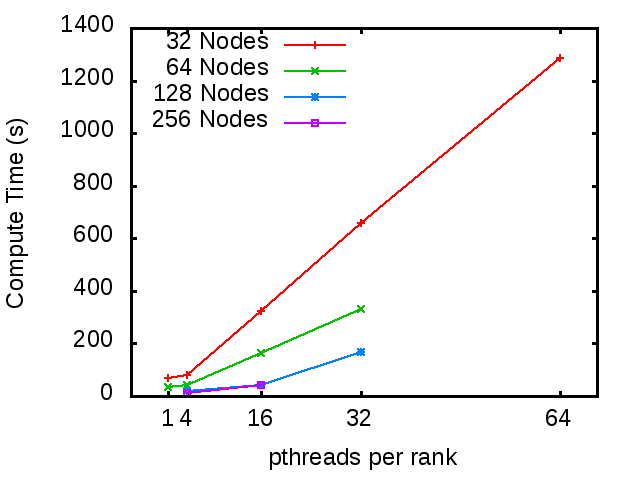
\includegraphics[width=\textwidth]{img/prMC-comp}

  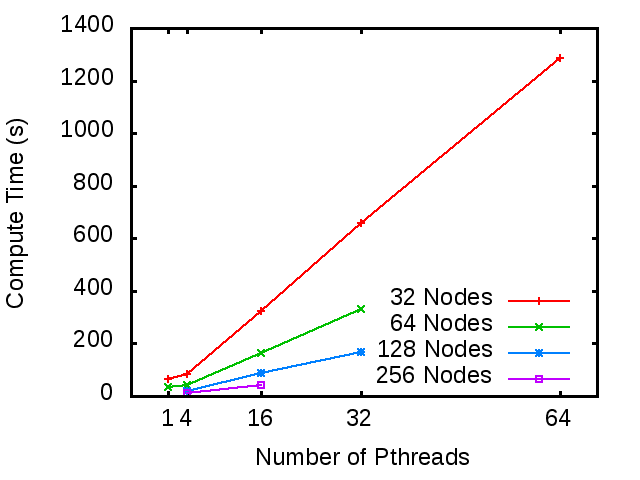
\includegraphics[width=\textwidth]{img/pr-comp}
  \captionof{figure}{Computation time for (top) 15 Monte Carlo steps and (bottom) 15 phase-field iterations.}
\end{minipage}
\end{center}

\begin{center}
\begin{minipage}{0.4\textwidth}\centering
  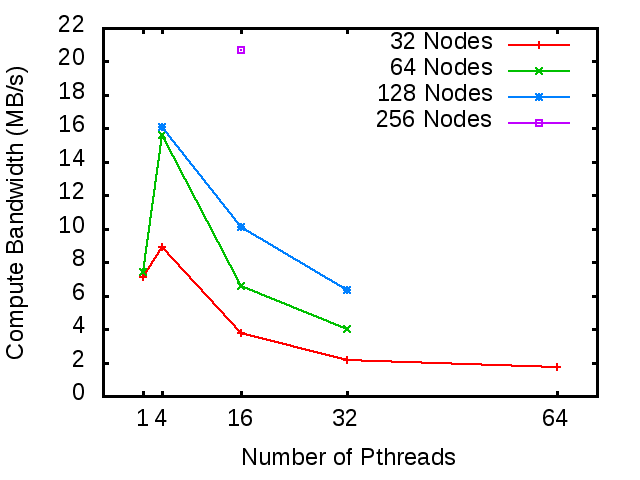
\includegraphics[width=\textwidth]{img/prMC-compBW}
  \captionof{figure}{Parallel I/O bandwidth writing $15^{\mathrm{th}}$ Monte Carlo step.}
\end{minipage}
\begin{minipage}{0.4\textwidth}\centering
  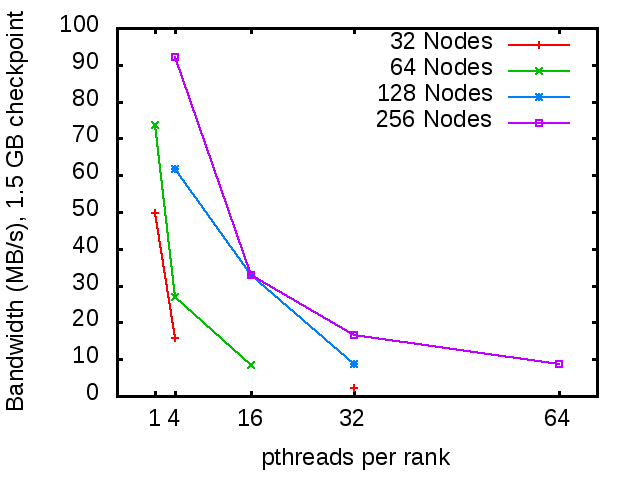
\includegraphics[width=\textwidth]{img/pr-compBW}
  \captionof{figure}{Parallel I/O bandwidth writing $15^{\mathrm{th}}$ phase-field iteration.}
\end{minipage}
\end{center}


\section{Conclusions}


\section{Contributions}
\begin{itemize}
 \item Kun Huang\\
	MC algorithm implementation and pthreading
 \item Trevor Keller\\
	Voronoi algorithm selection and implementation; parallel PF selection and implementation; MPI-IO algorithm design and implementation
 \item Congrui Li\\
	pthread PF and Voronoi
 \item Yixuan Tan\\
	MC algorithm selection and implementation
\end{itemize}

\label{LastPage}
\begin{footnotesize}
\begin{thebibliography}{1}
  \bibitem{Steinbach1999} I.~Steinbach and F.~Pezzolla. ``A generalized field method for multiphase transformations using interface fields.'' \emph{Physica D: Nonlinear Phenomena} \textbf{134} (1999) 385--393.
  \bibitem{Wright} S.A.~Wright, S.J.~Plimpton, T.P.~Swiler, R.M.~Fye, M.F.~Young, and E.A.~Holm. ``Potts-model grain growth simulations: Parallel algorithms and applications.'' \emph{SAND Report} (1997) 1925.
  \bibitem{Shim} Y.~Shim and J.G.~Amar. ``Synchronous sublattice algorithm for parallel kinetic Monte Carlo.'' \emph{arXiv preprint cond-mat} (2004) 0406379.
  \bibitem{Carothers2010} J.~Fu, N.~Liu, O.~Sahni, K.~Jansen, M.~Shephard, and C.D.~Carothers. ``Scalable parallel I/O alternatives for massively parallel partitioned solver systems.'' \emph{IEEE International Symposium on Parallel Distributed Processing} (2010) 1--8.
  \bibitem{Carothers2011} J.~Fu, M.~Min, R.~Latham, and C.D.~Carothers. ``Parallel I/O Performance for Application-Level Checkpointing on the Blue Gene/P System.'' \emph{CLUSTER} (2011) 465--473.
\end{thebibliography}
\end{footnotesize}
\end{multicols*}
\end{document}
